%%%%%%%%%%%%%%%%%%%%%%%%%%%%%%%%%%%%%%%%%%%%%%%%%%%%%%%%%%%%%%%%%
% MUW Presentation
% LaTeX Template
% Version 1.0 (27/12/2016)
%
% License:
% CC BY-NC-SA 4.0 (http://creativecommons.org/licenses/by-nc-sa/3.0/)
%
% Created by:
% Nicolas Ballarini, CeMSIIS, Medical University of Vienna
% nicoballarini@gmail.com
% http://statistics.msi.meduniwien.ac.at/
%
% Customized for UAH by:
% David F. Barrero, Departamento de Automática, UAH
%%%%%%%%%%%%%%%%%%%%%%%%%%%%%%%%%%%%%%%%%%%%%%%%%%%%%%%%%%%%%%%%%

\documentclass[10pt,compress]{beamer} % Change 10pt to make fonts of a different size
\mode<presentation>

\usepackage[spanish]{babel}
\usepackage{fontspec}
\usepackage{tikz}
\usepackage{etoolbox}
\usepackage{xcolor}
\usepackage{xstring}
\usepackage{listings}
\usepackage{multicol}
\usepackage{tabularx}
\usepackage{tikz}
\usetikzlibrary{matrix,chains,positioning,decorations.pathreplacing,arrows,shapes}

\usetheme{UAH}
\usecolortheme{UAH}
\setbeamertemplate{navigation symbols}{} 
\setbeamertemplate{caption}[numbered]

%%%%%%%%%%%%%%%%%%%%%%%%%%%%%%%%%%%%%%%%%%%%%%%%%%%%%%%%%%%%%%%%%
%% Presentation Info
\title[Pandas]{Pandas}
\author{\asignatura\\\carrera}
\institute{}
\date{Departamento de Automática}
%%%%%%%%%%%%%%%%%%%%%%%%%%%%%%%%%%%%%%%%%%%%%%%%%%%%%%%%%%%%%%%%%


%%%%%%%%%%%%%%%%%%%%%%%%%%%%%%%%%%%%%%%%%%%%%%%%%%%%%%%%%%%%%%%%%
%% Descomentar para habilitar barra de navegación superior
\setNavigation
%%%%%%%%%%%%%%%%%%%%%%%%%%%%%%%%%%%%%%%%%%%%%%%%%%%%%%%%%%%%%%%%%

%%%%%%%%%%%%%%%%%%%%%%%%%%%%%%%%%%%%%%%%%%%%%%%%%%%%%%%%%%%%%%%%%
%% Configuración de logotipos en portada
%% Opacidad de los logotipos
\newcommand{\opacidad}{1}
%% Descomentar para habilitar logotipo en pié de página de portada
\renewcommand{\logoUno}{Images/isg.png}
%% Descomentar para habilitar logotipo en pié de página de portada
%\renewcommand{\logoDos}{Images/CCLogo.png}
%% Descomentar para habilitar logotipo en pié de página de portada
%\renewcommand{\logoTres}{Images/ALogo.png}
%% Descomentar para habilitar logotipo en pié de página de portada
%\renewcommand{\logoCuatro}{Images/ELogo.png}
%%%%%%%%%%%%%%%%%%%%%%%%%%%%%%%%%%%%%%%%%%%%%%%%%%%%%%%%%%%%%%%%%

%%%%%%%%%%%%%%%%%%%%%%%%%%%%%%%%%%%%%%%%%%%%%%%%%%%%%%%%%%%%%%%%%
%% FOOTLINE
%% Comment/Uncomment the following blocks to modify the footline
%% content in the body slides. 


%% Option A: Title and institute
\footlineA
%% Option B: Author and institute
%\footlineB
%% Option C: Title, Author and institute
%\footlineC
%%%%%%%%%%%%%%%%%%%%%%%%%%%%%%%%%%%%%%%%%%%%%%%%%%%%%%%%%%%%%%%%%

\begin{document}

%%%%%%%%%%%%%%%%%%%%%%%%%%%%%%%%%%%%%%%%%%%%%%%%%%%%%%%%%%%%%%%%%
% Use this block for a blue title slide with modified footline
{\titlepageBlue
    \begin{frame}
        \titlepage
    \end{frame}
}

\institute{\asignatura}

\begin{frame}[plain]{}
	\begin{block}{Objectives}
		\begin{enumerate}
		\item Introduce Series and DataFrame data structures
		\item Understand Pandas features
		\item Fluent data manipulation with Pandas
		\item Data exploration
		\end{enumerate}
	\end{block}

   \begin{block}{Bibliography}
       Jake VanderPlas. \textit{Python Data Science Handbook}. Chapter 3. O'Reilly. \href{https://jakevdp.github.io/PythonDataScienceHandbook/}{(Link)}.
   \end{block}

\end{frame}

{
\disableNavigation{white}
\begin{frame}[shrink]{Table of Contents}
 \frametitle{Table of Contents}
 %\begin{multicols}{2}
 \tableofcontents
 %\end{multicols}
  % You might wish to add the option [pausesections]
\end{frame}
}

\section{Introduction}

\begin{frame}[fragile]{Introduction}
	\begin{columns}
 	   \column{0.6\textwidth}
		A DS/ML workflow needs more features
		\begin{itemize}
			\item Missing data
			\item Data input
			\item Operations on groups
			\item Label columns and rows
		\end{itemize}
		Pandas provides all those features, and more
		\begin{itemize}
			\item Pandas = \textbf{PAN}el \textbf{DA}ta \textbf{S}ystem
			\item Built on NumPy's ndarray
			\item Provides \alert{dataframes}
		\end{itemize}
		Pandas provides two main objects
		\begin{itemize}
			\item \texttt{Series} and \texttt{DataFrame}
		\end{itemize}

 	   \column{0.4\textwidth}
		\includegraphics[width=\textwidth]{figs/pandas.png}	

		\begin{block}{\footnotesize{Convention}}
		\vspace{-0.2cm} 
\begin{lstlisting}
import numpy as np
import pandas as pd
\end{lstlisting}
		\vspace{-0.2cm} 
		\end{block}

	\end{columns}
\end{frame}

\section{The Pandas \texttt{Series} object}

\begin{frame}[fragile]{The Pandas \texttt{Series} object (I)}
	\begin{columns}
 	   \column{0.6\textwidth}

		A \texttt{Series} is a one-dimensional array of indexed data
		\begin{itemize}
			\item NumPy arrays indices are implicit (i.e. its position)
			\item Series indices are explicit, and can be any type
		\end{itemize}
		Two attributes
		\begin{itemize}
			\item \texttt{values}: ndarray
			\item \texttt{index}: \texttt{pd.Index} object
		\end{itemize}
		Two indices
		\begin{itemize}
			\item Implicit: Regular index
			\item Explicit: Custom index
		\end{itemize}

 	   \column{0.4\textwidth}
	   \centering
      	\begin{tabularx}{2.7cm}{|c|c|}
			\hline
       		\textsc{Index} &  \textsc{Values}\\ \hline
       		\textit{'a'} & 0.25 \\
       		\textit{'b'} & 0.5  \\
       		\textit{'c'} & 0.75 \\
       		\textit{'d'} & 1 \\\hline
    	\end{tabularx}

		\bigskip

		\begin{exampleblock}{}
		\vspace{-0.2cm} 
			\begin{lstlisting}
data = pd.Series([0.25, 0.5, 0.75, 1.0])
data.values
data.index
data[1:3]
\end{lstlisting}
		\vspace{-0.2cm} 
		\end{exampleblock}
	\end{columns}
\end{frame}

\begin{frame}[fragile]{The Pandas \texttt{Series} object (II)}
	\begin{columns}
 	   \column{0.8\textwidth}
		\begin{exampleblock}{\footnotesize{Custom indices}}
		\vspace{-0.2cm} 
			\begin{lstlisting}
In[1] : data = pd.Series([0.25, 0.5, 0.75, 1.0],
                 index=['a', 'b', 'c', 'd'])
In [2]: data
Out[1]: 
   a    0.25
   b    0.50
   c    0.75
   d    1.00
dtype: float64

In [3]: data['a']
Out[2]: 0.25
In [4]: data[0]
Out[3]: 0.25
\end{lstlisting}
		\vspace{-0.2cm} 
		\end{exampleblock}
	\end{columns}
\end{frame}

\section{The Pandas \texttt{DataFrame} object}
\subsection{Dataframe concept}

\begin{frame}{The Pandas \texttt{DataFrame} object}{Dataframe concept (I)}
	\begin{columns}
 	   \column{0.5\textwidth}
		A \texttt{DataFrame} is a 2-D tabular data structure
		\begin{itemize}
			\item Similar to a spreadsheet
			\item Homogeneous columns
			\item Heterogeneous rows
		\end{itemize}
		Two read-only attributes, both \texttt{pd.Index}
		\begin{itemize}
			\item \texttt{index}: Rows
			\item \texttt{columns}: Columns
		\end{itemize}

 	   \column{0.4\textwidth}
		\centering \includegraphics[width=\textwidth]{figs/structure_table.jpg}\\
		%\centering 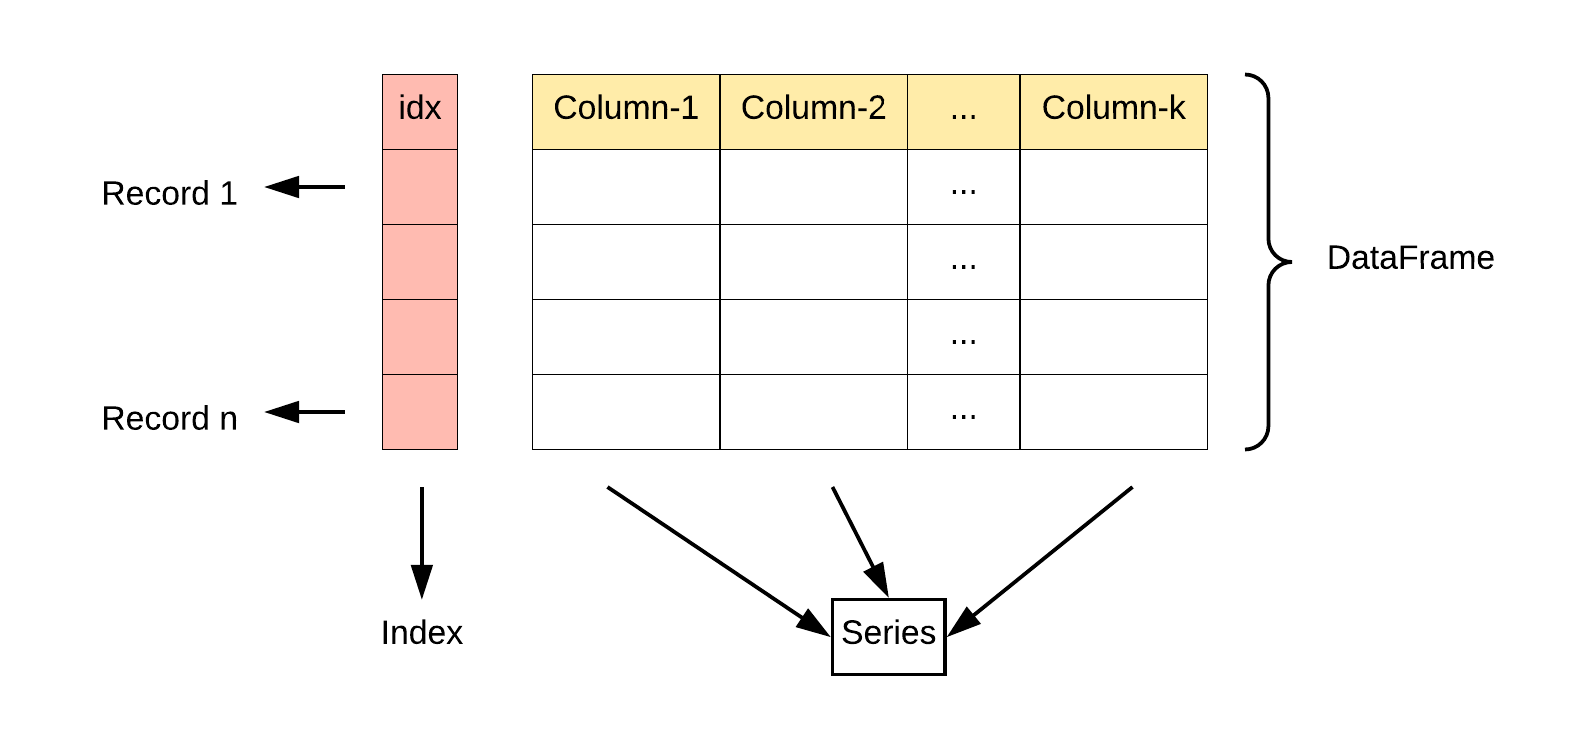
\includegraphics[width=\textwidth]{figs/dataframe.png}\\
		%\tiny \href{https://www.jiyik.com/w/pandas/pandas-dataframe}{(Source)}
		\tiny \href{https://www.tutorialspoint.com/python\_pandas/python\_pandas\_dataframe.htm}{(Source)}
	\end{columns}
\end{frame}

\begin{frame}[fragile]{The Pandas \texttt{DataFrame} object}{Dataframe concept (II)}
	\begin{columns}
	   \column{\textwidth}
		\begin{exampleblock}{\footnotesize{DataFrame example}}
		\vspace{-0.2cm} 
			\begin{lstlisting}
In [1]:  import seaborn as sns

In [2]:  iris = sns.load_dataset('iris')
In [3]:  iris.head()

Out[1]:
sepal_length  sepal_width  petal_length  petal_width species
0           5.1          3.5           1.4          0.2  setosa
1           4.9          3.0           1.4          0.2  setosa
2           4.7          3.2           1.3          0.2  setosa
3           4.6          3.1           1.5          0.2  setosa
4           5.0          3.6           1.4          0.2  setosa
In [246]: iris.columns
Out[246]: 
Index(['sepal_length', 'sepal_width', 'petal_length', 
        'petal_width', 'species'], dtype='object')
\end{lstlisting}
		\vspace{-0.2cm} 
		\end{exampleblock}
	\end{columns}
\end{frame}

\subsection{Constructing \texttt{DataFrame} objects}
\begin{frame}[fragile]{The Pandas \texttt{DataFrame} object}{Constructing \texttt{DataFrame} objects (I)}
	Manual initialization
	\begin{itemize}
		\item From a single \texttt{Series} object\\
		\texttt{pd.DataFrame(population, columns=['population'])}
		\item From several \texttt{Series} objects\\
		\texttt{pd.DataFrame({'population': population,
		                       'area': area})}
		\item From a dictionary\\
	    \texttt{pd.DataFrame([\{'a': 0, 'b': 0\}, \{'a': 1, 'b': 2\}])}
		\item From a NumPy 2-D array\\
		\texttt{pd.DataFrame(np.random.rand(3, 2), \\columns=['foo', 'bar'], index=['a', 'b', 'c'])}
	\end{itemize}
\end{frame}

\begin{frame}[fragile]{The Pandas \texttt{DataFrame} object}{Constructing \texttt{DataFrame} objects (II)}
	Read from a file
	\begin{itemize}
		\item CSV (very common!!!): \texttt{pd.read\_csv('filename.csv')}
		\item Excel:\\
		\texttt{pd.read\_excel('filename.xlsx', sheetname='mysheet')}
	\end{itemize}

	\begin{exampleblock}{CSV example}
		\begin{lstlisting}
# This CSV file contains data about weights and heights
"id", "weight","height","sex",  "race"
1,    143.5,   81.6,    "Female","White"
2,    109.1,   83.7,    "Female","Black"
4,    104.8,   54.6,    "Female","Hisp"
7,    130.2,   81.7,    "Male",  "White"
\end{lstlisting}
	\end{exampleblock}
	CVS can be exported from MS Excel or programatically
\end{frame}

\section{Data indexing and selection}
\subsection{\texttt{Series}}

\begin{frame}[fragile]{Data indexing and selection}{\texttt{Series}}
	\begin{columns}
 	   \column{0.5\textwidth}
		\begin{exampleblock}{Dictionary-like syntax}
		\vspace{-0.2cm} 
			\begin{lstlisting}
>> data = pd.Series([0.25, 0.5, 0.75, 1.0], index=['a', 'b', 'c', 'd'])

>> 'a' in data
True

>> data.keys()
Index(['a', 'b', 'c'], dtype='object')

>> list(data.items())
[('a', 0.25), ('b', 0.5), ('c', 0.75)]

>> data['e'] = 1.25
\end{lstlisting}
			\vspace{-0.2cm} 
		\end{exampleblock}

		\column{0.5\textwidth}
		\begin{exampleblock}{Array-like syntax}
			\vspace{-0.2cm} 
			\begin{lstlisting}
>> data['a':'c'] #Explicit index
   a    0.25
   b    0.50
   c    0.75
dtype: float64
>> data[0:2] # Implicit index
   a    0.25
   b    0.50
dtype: float64
>> data[data>0.5] # Masking
   c    0.75
   d    1.00
dtype: float64
>> data[['b','c']] # Fancy index
   b    0.5
   c    0.75
dtype: float64
\end{lstlisting}
			\vspace{-0.2cm} 
		\end{exampleblock}
	\end{columns}
\end{frame}

\begin{frame}[fragile]{Data indexing and selection}{\texttt{DataFrame}}
	\begin{columns}
 	   \column{0.5\textwidth}
		\begin{exampleblock}{Dictionary-like syntax}
		\vspace{-0.2cm} 
			\begin{lstlisting}
>> data['area']
>> data.area
>> data.area is data['area']
True
>> data['density'] = data['pop']/data['area']
			\end{lstlisting}
			\vspace{-0.2cm} 
		\end{exampleblock}

		\column{0.5\textwidth}
		\begin{exampleblock}{Array-like syntax}
		\vspace{-0.2cm} 
			\begin{lstlisting}
>> data.values # Get values array
>> data.T # Transpose
>> data[0] # First row
>> data['area'] # Area column
\end{lstlisting}
			\vspace{-0.2cm} 
		\end{exampleblock}
	\end{columns}

	\bigskip

	Remember indexing conventions
	\begin{itemize}
		\item Indexing refers to columns (\texttt{data['area']})
		\item Slicing refers to rows (\texttt{data['Florida':'Illinois']})
		\item Masking refers to rows (\texttt{data[data.density > 100]})
	\end{itemize}
\end{frame}

\subsection{Loc, iloc and ix}

\begin{frame}[fragile]{Data indexing and selection}{loc, iloc and ix}
	\begin{columns}
 	   \column{0.5\textwidth}
	Two types of indices in Pandas
	\begin{itemize}
		\item Explicit and implicit
		\item Indexing (\texttt{data[0]}) is explit
		\item Slicing (\texttt{data[:2]}) is implicit (Python-like)
		\item Source of troubles!
	\end{itemize}
	Pandas makes explicit the used scheme
	\begin{itemize}
		\item \texttt{loc}: Explicit index
		\item \texttt{iloc}: Implicit index
		\item \texttt{ix}: Hybrid
	\end{itemize}
 	   \column{0.5\textwidth}
		\begin{exampleblock}{}
		\vspace{-0.2cm} 
			\begin{lstlisting}
# Series
>> serie.loc[1]
>> serie.loc[1:3]
>> serie.iloc[1]
>> serie.iloc[1:3]

# Dataframes
>> df.iloc[:3, :2]
>> df.loc[:'illinois', :'pop']
>> df.ix[:3, :'pop']
>> df.loc[df.data>100, ['pop', 'density']]
>> df.iloc[0, 2] = 90
\end{lstlisting}
		\end{exampleblock}
	\end{columns}
\end{frame}

\section{Operating on data}
\subsection{Overview}

\begin{frame}[fragile]{Operating on data}{Overview (I)}
	\begin{columns}
 	   \column{0.4\textwidth}
		Pandas fully supports NumPy's ufuncs
		\begin{itemize}
			\item Efficient computations
		\end{itemize}
		Additional Pandas features
		\begin{itemize}
			\item Index and column name preservation
			\item Index aligning
			\item Easy data combination
		\end{itemize}

 	   \column{0.6\textwidth}
		\begin{exampleblock}{}
		\vspace{-0.2cm} 
			\begin{lstlisting}
>> rng = np.random.RandomState(42)
>> df = pd.DataFrame(rng.randint(0, 10, (3,4)))
>> df = pd.DataFrame(rng.randint(0, 10, (3,4)), columns=['A', 'B', 'C', 'D'])
>> print(df)
   A  B  C  D
0  7  2  5  4
1  1  7  5  1
2  4  0  9  5
>> np.sin(df * np.pi / 4)
   A       B    C    D
0 -7.07e-01  1.0 -0.7  1.22e-16
1  7.07e-01 -0.7 -0.7  7.07e-01
2  1.22e-16  0.0  0.7 -7.07e-01
\end{lstlisting}
			\vspace{-0.2cm} 
		\end{exampleblock}
	\end{columns}
\end{frame}

\begin{frame}[fragile]{Operating on data}{Overview (II)}
	\begin{columns}
 	   \column{0.8\textwidth}
		\begin{exampleblock}{Index preservation}
		\vspace{-0.2cm} 
			\begin{lstlisting}
>> A = pd.Series([2, 4, 6], index=[0, 1, 2])
>> B = pd.Series([1, 3, 5], index=[1, 2, 3])
>> A + B
   0    NaN
   1    5.0
   2    9.0
   3    NaN
dtype: float64
>> A.add(B, fill_value=0)
   0    2.0
   1    5.0
   2    9.0
   3    5.0
dtype: float64
\end{lstlisting}
			\vspace{-0.2cm} 
		\end{exampleblock}
	\end{columns}
\end{frame}

\subsection{Missing data}

\begin{frame}[fragile]{Operating on data}{Missing data (I)}
	NumPy supports missing data in floating-point data
	\begin{itemize}
		\item Specific value defined by IEEE
		\item Available as \texttt{np.nan}
	\end{itemize}
	Pandas supports missing data through two mechanisms
	\begin{itemize}
		\item \texttt{None} object, interpreted as NaN (\texttt{Not a Number})
		\item \texttt{np.nan}: for floating-point data
		\item Almost automatic NaN handling (types upcast)
	\end{itemize}

	\begin{columns}
 	   \column{0.55\textwidth}
		\begin{exampleblock}{}
		\vspace{-0.2cm} 
			\begin{lstlisting}
>> pd.Series([1, np.nan, 2, None])
   0    1.0
   1    NaN
   2    2.0
   3    NaN
dtype: float64
\end{lstlisting}
			\vspace{-0.2cm} 
		\end{exampleblock}
	\end{columns}
\end{frame}

\begin{frame}[fragile]{Pandas}{Missing data (II)}
	\begin{columns}
 	   \column{0.5\textwidth}
		Useful functions for missing data
		\begin{itemize}
			\item \texttt{isnull()}: Boolean mask with missing data
			\item \texttt{notnull()}: Opposite of isnull()
			\item \texttt{dropna()}: Filtered data
			\item \texttt{fillna()}: NaNs filled
		\end{itemize}

 	   \column{0.5\textwidth}
		\begin{exampleblock}{}
		\vspace{-0.2cm} 
			\begin{lstlisting}
>> data = pd.Series([1, np.nan, 'hello', None])
>> data[data.notnull()]
   0        1
   2    hello
dtype: object

>> data.dropna()
   0        1
   2    hello
dtype: object

>> data.fillna(0)
   0        1
   1        0
   2    hello
   3        0
dtype: object
\end{lstlisting}
			\vspace{-0.2cm} 
		\end{exampleblock}
	\end{columns}
\end{frame}

\section{Combining datasets}
\subsection{\texttt{pd.concat()}}

\begin{frame}[fragile]{Combining datasets}{\texttt{pd.concat()} (I)}
	Many times we need to combine two or more datasets
	\begin{itemize}
		\item Pandas provides \texttt{pd.concat()}, \texttt{append()} and \texttt{pd.merge()}
	\end{itemize}

	\begin{columns}
    \column{0.9\textwidth}
	\begin{block}{pd.concat() signature}
	\vspace{-0.2cm} 
		\begin{lstlisting}
pd.concat(objs, axis=0, join='outer', join_axes=None, ignore_index=False, keys=None, levels=None, names=None, verify_integrity=False, copy=True)
\end{lstlisting}
		\vspace{-0.2cm} 
	\end{block}
	\end{columns}

	By default, \texttt{pd.concat()} joins rows preserving index
	\begin{itemize}
		\item \texttt{axis}: Join columns (\texttt{axis=1})
		\item \texttt{verify\_integrity}: Raise error if duplicates (\texttt{verify\_integrity=True})
		\item \texttt{ignore\_index}: Create new index (\texttt{ignore\_index=True})
		\item \texttt{join}: Can be 'outer' (union) or 'inner' (intersection)
	\end{itemize}
\end{frame}

\begin{frame}[fragile]{Combining datasets}{\texttt{pd.concat()} (II)}
	\begin{columns}
 	   \column{1.1\textwidth}
		\begin{exampleblock}{}
		\vspace{-0.2cm} 
			\begin{lstlisting}
>> df1 = pd.DataFrame([{'A': 'A0', 'B': 'B0'}, {'A': 'A1', 'B': 'B1'}])
>> df2 = pd.DataFrame([{'A': 'A2', 'B': 'B2'}, {'A': 'A3', 'B': 'B3'}])

>> print(df1), print(df2); print(pd.concat([df1, df2]))
   A   B        A   B       A   B
0  A0  B0    0  A2  B2   0  A0  B0
1  A1  B1    1  A3  B3   1  A1  B1
                         0  A2  B2
                         1  A3  B3
>> pd.concat([df1, df2], axis=1)
   A   B   A   B
0  A0  B0  A2  B2
1  A1  B1  A3  B3
>> df1.append(df2)
\end{lstlisting}
			\vspace{-0.2cm} 
		\end{exampleblock}
		\end{columns}
\end{frame}

\subsection{\texttt{pd.merge()}}

\begin{frame}[fragile]{Combining datasets}{\texttt{pd.merge()} (I)}
	Merging based on relational algebra
	\begin{itemize}
		\item Similar to databases tables joins
		\item Pretty intelligent figuring out the desired output
		\item By default, join dataframes using shared columns names
	\end{itemize}
\end{frame}

\begin{frame}[fragile]{Combining datasets}{\texttt{pd.merge()} (II)}
	\scriptsize{
	\begin{columns}
    \column{0.45\textwidth}
		\begin{exampleblock}{One-to-one}
		\vspace{-0.2cm} 
		\begin{lstlisting}
>> print(df1); print(df2)
 employee        group
0     Bob   Accounting
1    Jake  Engineering
2    Lisa  Engineering
3     Sue           HR
 employee  hire_date
0    Lisa       2004
1     Bob       2008
2    Jake       2012
3     Sue       2014
>> print(pd.merge(df1, df2))
 employee group  hire_date
0     Bob Accounting  2008
1    Jake Engineering 2012
2    Lisa Engineering 2004
3     Sue HR          2014
\end{lstlisting}
		\vspace{-0.2cm} 
		\end{exampleblock}

    \column{0.6\textwidth}
		\begin{exampleblock}{Many-to-one}
		\vspace{-0.2cm} 
		\begin{lstlisting}
>> print(df3); print(df4)
  employee  group  hire_date
0      Bob   Accounting  2008
1     Jake  Engineering  2012
2     Lisa  Engineering  2004
3      Sue           HR  2014
         group  supervisor
0   Accounting  Carly
1  Engineering  Guido
2           HR  Steve
>> print(pd.merge(df3, df4))
employee  group hire_date  supervisor
0  Bob   Accounting  2008  Carly
1 Jake  Engineering  2012  Guido
2 Lisa  Engineering  2004  Guido
3  Sue           HR  2014  Steve
\end{lstlisting}
		\vspace{-0.2cm} 
		\end{exampleblock}
	\end{columns}
	}
\end{frame}

\begin{frame}[fragile]{Combining datasets}{\texttt{pd.merge()} (III)}
	\scriptsize{
	\begin{columns}
    \column{0.9\textwidth}
		\begin{exampleblock}{\footnotesize{Many-to-many}}
		\vspace{-0.2cm} 
		\begin{lstlisting}
>> print(df1); print(df5)
  employee        group              group        skills
0      Bob   Accounting     0   Accounting          math
1     Jake  Engineering     1   Accounting  spreadsheets
2     Lisa  Engineering     2  Engineering        coding
3      Sue           HR     3  Engineering         linux
                            4           HR  spreadsheets
                            5           HR  organization
>> pd.merge(df1, df5)
   employee        group        skills
0      Bob   Accounting          math
1      Bob   Accounting  spreadsheets
2     Jake  Engineering        coding
3     Jake  Engineering         linux
4     Lisa  Engineering        coding
5     Lisa  Engineering         linux
6      Sue           HR  spreadsheets
7      Sue           HR  organization
\end{lstlisting}
		\vspace{-0.2cm} 
		\end{exampleblock}
	\end{columns}
	}
\end{frame}

\begin{frame}[fragile]{Combining datasets}{\texttt{pd.merge()} (IV)}
	\begin{columns}
    \column{\textwidth}
	\begin{block}{pd.merge() signature}
		\vspace{-0.2cm} 
		\begin{lstlisting}
pd.merge(left, right, how='inner', on=None, left_on=None, right_on=None, left_index=False, right_index=False, sort=False, suffixes=('_x', '_y'), copy=True, indicator=False, validate=None)
\end{lstlisting}
		\vspace{-0.2cm} 
		\end{block}
	\end{columns}
	
	\bigskip

	Arguments:
	\begin{itemize}
		\item \texttt{on}: Key column name
		\item \texttt{left\_on}: Left table key column name
		\item \texttt{right\_on}: Right table key column name
		\item \texttt{how}: Set arithmetic, \texttt{'inner'} (default, intersection), \texttt{'outer'} (union, fills missings with NaNs), \texttt{'left'} (left entries), \texttt{'right'} (right entries)
	\end{itemize}

\end{frame}

\begin{frame}[fragile]{Combining datasets}{\texttt{pd.merge()} (V)}
	\begin{columns}
    \column{\textwidth}
	\begin{exampleblock}{}
	\vspace{-0.2cm} 
		\begin{lstlisting}
>>> A              >>> B
    lkey value         rkey value
0   foo  1         0   foo  5
1   bar  2         1   bar  6
2   baz  3         2   qux  7
3   foo  4         3   bar  8

>>> A.merge(B, left_on='lkey', right_on='rkey', how='outer')
    lkey  value_x  rkey  value_y
0   foo   1        foo   5
1   foo   4        foo   5
2   bar   2        bar   6
3   bar   2        bar   8
4   baz   3        NaN   NaN
5   NaN   NaN      qux   7
\end{lstlisting}
		\vspace{-0.2cm} 
	\end{exampleblock}
	\end{columns}
\end{frame}

\section{Aggregation in Pandas}

\begin{frame}[fragile]{Aggregation in Pandas (I)}
	\begin{columns}
 	   \column{0.4\textwidth}
		The first step in data analysis is summarization
		\begin{itemize}
			\item First contact with data
			\item Insight to the dataset
		\end{itemize}
		Aggregation methods
		\begin{itemize}
			\item Applied to columns
		\end{itemize}
	
 	   \column{0.6\textwidth}
      	\begin{tabularx}{\textwidth}{rl}
			\hline
       		\textsc{Aggregation} &  \textsc{Description}\\ \hline
       		\texttt{count()}    & 	Total number of items \\
       		\texttt{first()}, \texttt{last()} & First and last item \\
       		\texttt{mean()}, \texttt{median()} & Mean and median \\
       		\texttt{min()}, \texttt{max()} & Minimum and maximum \\
       		\texttt{std()}, \texttt{var()} & Standard dev. and variance \\
       		\texttt{mad()} & Mean absolute deviation \\
       		\texttt{prod()} & Product of all items \\
       		\texttt{sum()} & Sum of all items \\
       		\texttt{describe()} & Data summary \\\hline
    	\end{tabularx}
	\end{columns}
\end{frame}

\begin{frame}[fragile,plain]
	\scriptsize{
	%\vspace{-0.5cm}
	\begin{columns}
 	   \column{\textwidth}
		\begin{exampleblock}{}
		\vspace{-0.2cm} 
			\begin{lstlisting}
>> import seaborn as sns
>> planets = sns.load_dataset('planets')
>> planets.head()
            method number orbital_period mass distance  year
0  Radial Velocity 1      269.300        7.10    77.40  2006
1  Radial Velocity 1      874.774        2.21    56.95  2008
2  Radial Velocity 1      763.000        2.60    19.84  2011
3  Radial Velocity 1      326.030       19.40   110.62  2007
4  Radial Velocity 1      516.220       10.50   119.47  2009
>> planets.dropna().describe()
       number  orbital_period    mass  distance      year
count  498.00      498.000000  498.00  498.0000   498.000
mean     1.73      835.778671    2.50   52.0682  2007.377
std      1.17     1469.128259    3.63   46.5960     4.167
min      1.00        1.328300    0.00    1.3500  1989.000
25%      1.00       38.272250    0.21   24.4975  2005.000
50%      1.00      357.000000    1.24   39.9400  2009.000
75%      2.00      999.600000    2.86   59.3325  2011.000
max      6.00    17337.500000   25.00  354.0000  2014.000
>> planets.mean()
number               1.785507
orbital_period    2002.917596
mass                 2.638161
distance           264.069282
year              2009.070531
dtype: float64
\end{lstlisting}
			\vspace{-0.2cm} 
		\end{exampleblock}
	\end{columns}
	}
\end{frame}

\subsection{Grouping in Pandas}
\begin{frame}{Grouping in Pandas (I)}
		Aggregation is generally used ...
		\begin{itemize}
			\item ... good to operate with the whole dataset ...
			\item ... but also is is usually insufficient
		\end{itemize}
		We need conditional aggregations
		\begin{itemize}
			\item Aggregate conditionally on some label
		\end{itemize}
		This is done with the operation \texttt{groupby} (yes, that name comes from SQL)
		\begin{itemize}
			\item Example: \texttt{df.groupby("key")}
		\end{itemize}
		Three tasks in one step
		\begin{enumerate}
			\item \textit{Split}: Break up dependening on a key
			\item \textit{Apply}: Compute some function
			\item \textit{Combine}: Merge results into an output
		\end{enumerate}
\end{frame}

\begin{frame}{Grouping in Pandas (II)}
	\centering \includegraphics[width=0.9\textwidth]{figs/03.08-split-apply-combine.png}\\
\end{frame}

\begin{frame}[fragile]{Grouping in Pandas (III)}
	\vspace{-0.5cm}
	\begin{columns}
 	   \column{\textwidth}
		\begin{exampleblock}{}
		\vspace{-0.2cm} 
			\begin{lstlisting}
>> df = pd.DataFrame({'key': ['A', 'B', 'C', 'A', 'B', 'C'],
                      'data': range(6)})
>> print(df)
  key  data
0   A     0
1   B     1
2   C     2
3   A     3
4   B     4
5   C     5
>> df.groupby('key')
<pandas.core.groupby.groupby.DataFrameGroupBy object at 0x102685438>
>> df.groupby('key').sum()
     data
key      
A       3
B       5
C       7
\end{lstlisting}
			\vspace{-0.2cm} 
		\end{exampleblock}
	\end{columns}
\end{frame}

\begin{frame}{Grouping in Pandas (IV)}
	Several mapping methods available
	\begin{itemize}
		\item List\\
			  \texttt{df.groupby([2,3,4,1]).sum()}
		\item Dictionary \\
			  \texttt{df.groupby({'A': 'vowel', 'B': 'consonant', 'C': 'vowel'})}
		\item Python function \\
			  \texttt{df.groupby(str.lower)}
		\item Multiple keys \\
		      \texttt{planets.groupby(['method', 'year'])}
		\item Mixed keys \\
		      \texttt{df.groupby(['key1', 'key2', str.lower])}
	\end{itemize}
\end{frame}

\begin{frame}{Grouping in Pandas (V)}
	The method \texttt{groupby()} returns an object \texttt{groupby}
	\begin{itemize}
		\item Basicly, it is a collection of dataframes\\
		      \texttt{planets.groupby('method').get\_group('Transit')}
		\item Column selection as dataframe\\
		      \texttt{planets.groupby('method')['year']}
	\end{itemize}
	Interesting groupby attribute, \texttt{groups}
	\begin{itemize}
		\item Dictionary with groups\\
		      \texttt{planets.groupby('method').groups}
		\item Compatible with the \texttt{len()} method\\
		      \texttt{len(planets.groupby('method'))}
	\end{itemize}
\end{frame}

\begin{frame}{Grouping in Pandas (VI)}
	Usual operations with groupings
	\begin{itemize}
		\item Aggregation: \\
			\texttt{df.groupby('key').aggregate(['min', np.median, max])}\\
			\texttt{df.groupby('key').aggregate({'data1': 'min', 'data2': 'max'})}
		\item Filtering: \\
			\texttt{planets.groupby('method').filter(lambda x: x['distance'].mean() > 50.)}
		\item Transformation: \\
			\texttt{df.groupby('key').transform(lambda x: x - x.mean())}
	\end{itemize}
	Apply(): Apply arbitrary function and combine results
		\begin{itemize}
			\item Takes a function as argument that takes a DataFrame
			\item[] \texttt{planets.groupby("method").apply(lambda x: x / x.sum())}
		\end{itemize}
\end{frame}

\begin{frame}[fragile]{Grouping in Pandas (VII)}
	\begin{columns}
    \column{0.8\textwidth}
	\begin{exampleblock}{Grouping by decade}
	\vspace{-0.2cm} 
		\begin{lstlisting}
decade = 10 * (planets['year'] // 10)
decade = decade.astype(str) + 's'
decade.name = 'decade'
planets.groupby(['method', decade])['number'].sum().unstack().fillna(0)
\end{lstlisting}
		\vspace{-0.2cm} 
	\end{exampleblock}
	\end{columns}
\end{frame}

\end{document}
